\documentclass[10pt]{beamer}
\usetheme{m}
\usecolortheme[RGB={1,1,1}]{structure}
\usepackage{booktabs}
\usepackage[scale=2]{ccicons}
\usepackage{pgfplots}
\usepgfplotslibrary{dateplot}
\usepackage[utf8x]{inputenc}
\usepackage{ucs}
\usepackage[spanish]{babel}
\usepackage{amsmath}
\usepackage{amsfonts}
\usepackage{amssymb}
\usepackage{graphicx}
\title{Identificación de proteínas y rutas metabólicas asociadas a la respuesta neuroprotectora mediada por la tibolona en astrocitos bajo un modelo inflamatorio inducido.\vspace{-0.75\baselineskip}}
\date{Agosto 14, 2015}
\author{Daniel Camilo Osorio}
\institute{\textbf{Maestría en Bioinformática}\\ Universidad Nacional de Colombia\\\textbf{Laboratorio de Bioquímica Computacional y Bioinformática} \\ Pontificia Universidad Javeriana}
%\titlegraphic{\hfill
\includegraphics[height=1.5cm]{imagenes/VUNAL}}
\begin{document}
\maketitle
\begin{frame}
\frametitle{Proteinas}
\begin{center}
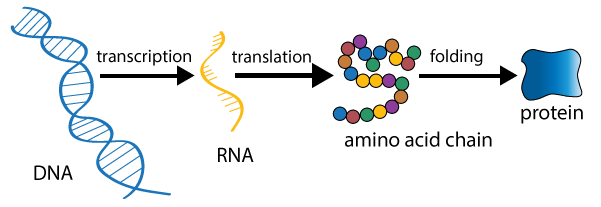
\includegraphics[width=10cm]{imagenes/BCD}
\end{center}
\begin{flushright}
\tiny{© Bio-Social Methods Collaborative 2013 The Regents of the University of Michigan}
\end{flushright}
\begin{itemize}
\item Están determinadas mayoritariamente por la genética de los organismos.
\pause
\item Son los componentes principales de las rutas metabólicas de las células.
\end{itemize}
\end{frame}
\begin{frame}
\frametitle{Proteínas}
\begin{center}
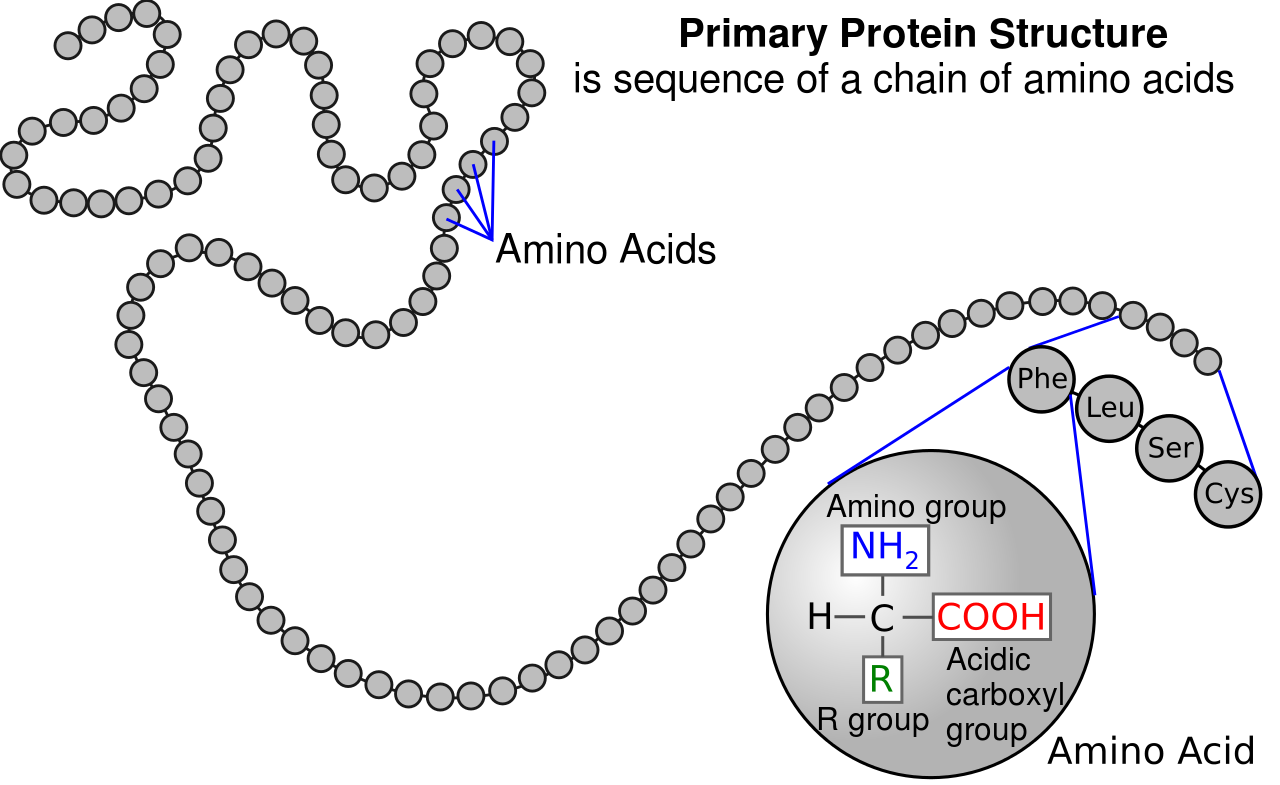
\includegraphics[width=8cm]{imagenes/AA}
\end{center}
\begin{flushright}
\tiny{© Bio-Social Methods Collaborative 2013 The Regents of the University of Michigan}
\end{flushright}
\begin{itemize}
\item Son moléculas formadas por cadenas lineales de aminoácidos.
\pause
\item Realizan funciones enzimáticas, estructurales y de transducción de señales entre otras.
\pause
\item El conjunto de las proteínas expresadas en una circunstancia determinada es denominado \emph{proteoma}.
\end{itemize}
\end{frame}
\begin{frame}
\frametitle{Proteoma}
\begin{center}
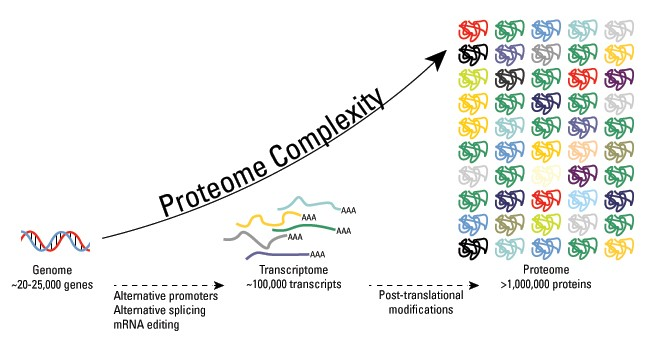
\includegraphics[width=10cm]{imagenes/Proteome}
\end{center}
\begin{itemize}
\item Es el equivalente proteínico del \emph{genoma}.
\pause
\item Es la totalidad de proteínas expresadas en una célula bajo ciertas condiciones ó etapas de desarrollo específicas.
\end{itemize}
\end{frame}
\begin{frame}
\frametitle{Métodos para caracterización de proteomas}
\begin{center}
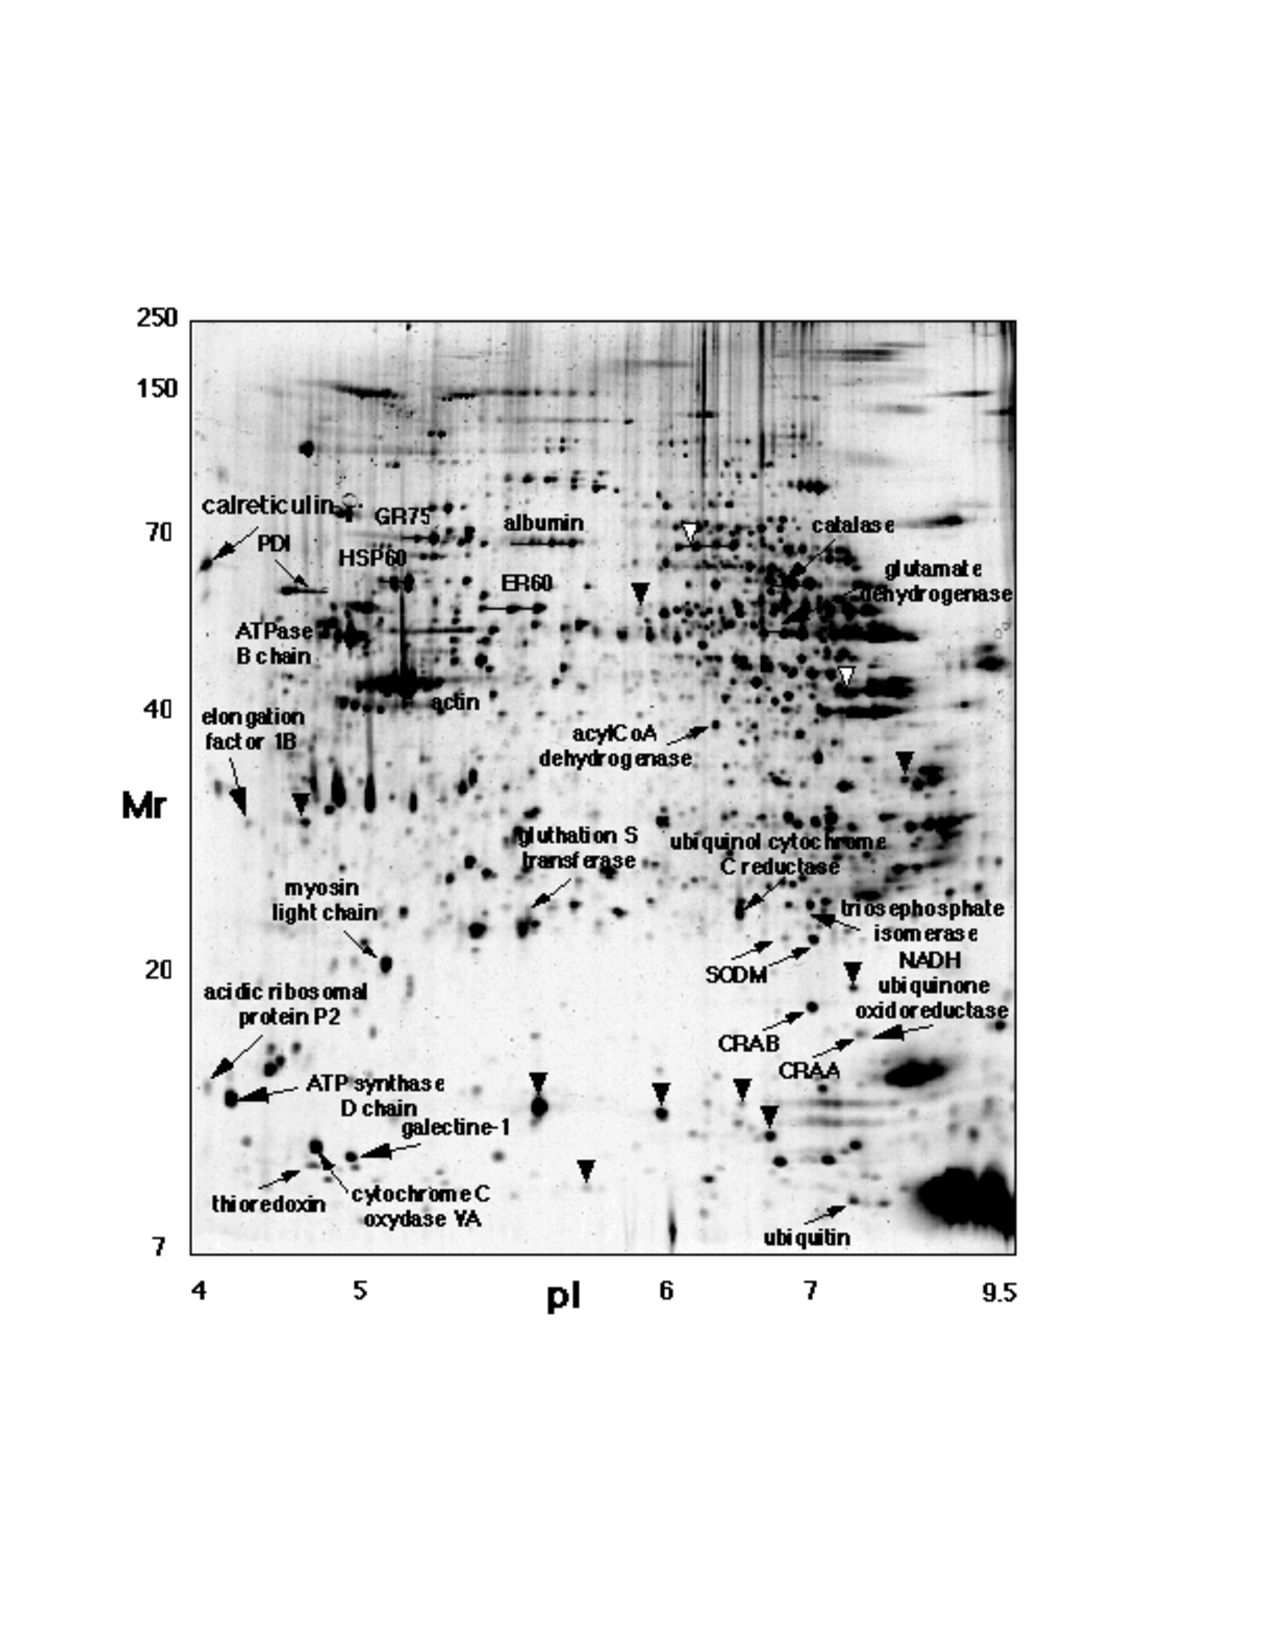
\includegraphics[width=7cm]{imagenes/2DPAGE}
\end{center}
\end{frame}
\begin{frame}
\frametitle{Métodos para caracterización de proteomas}
\begin{center}
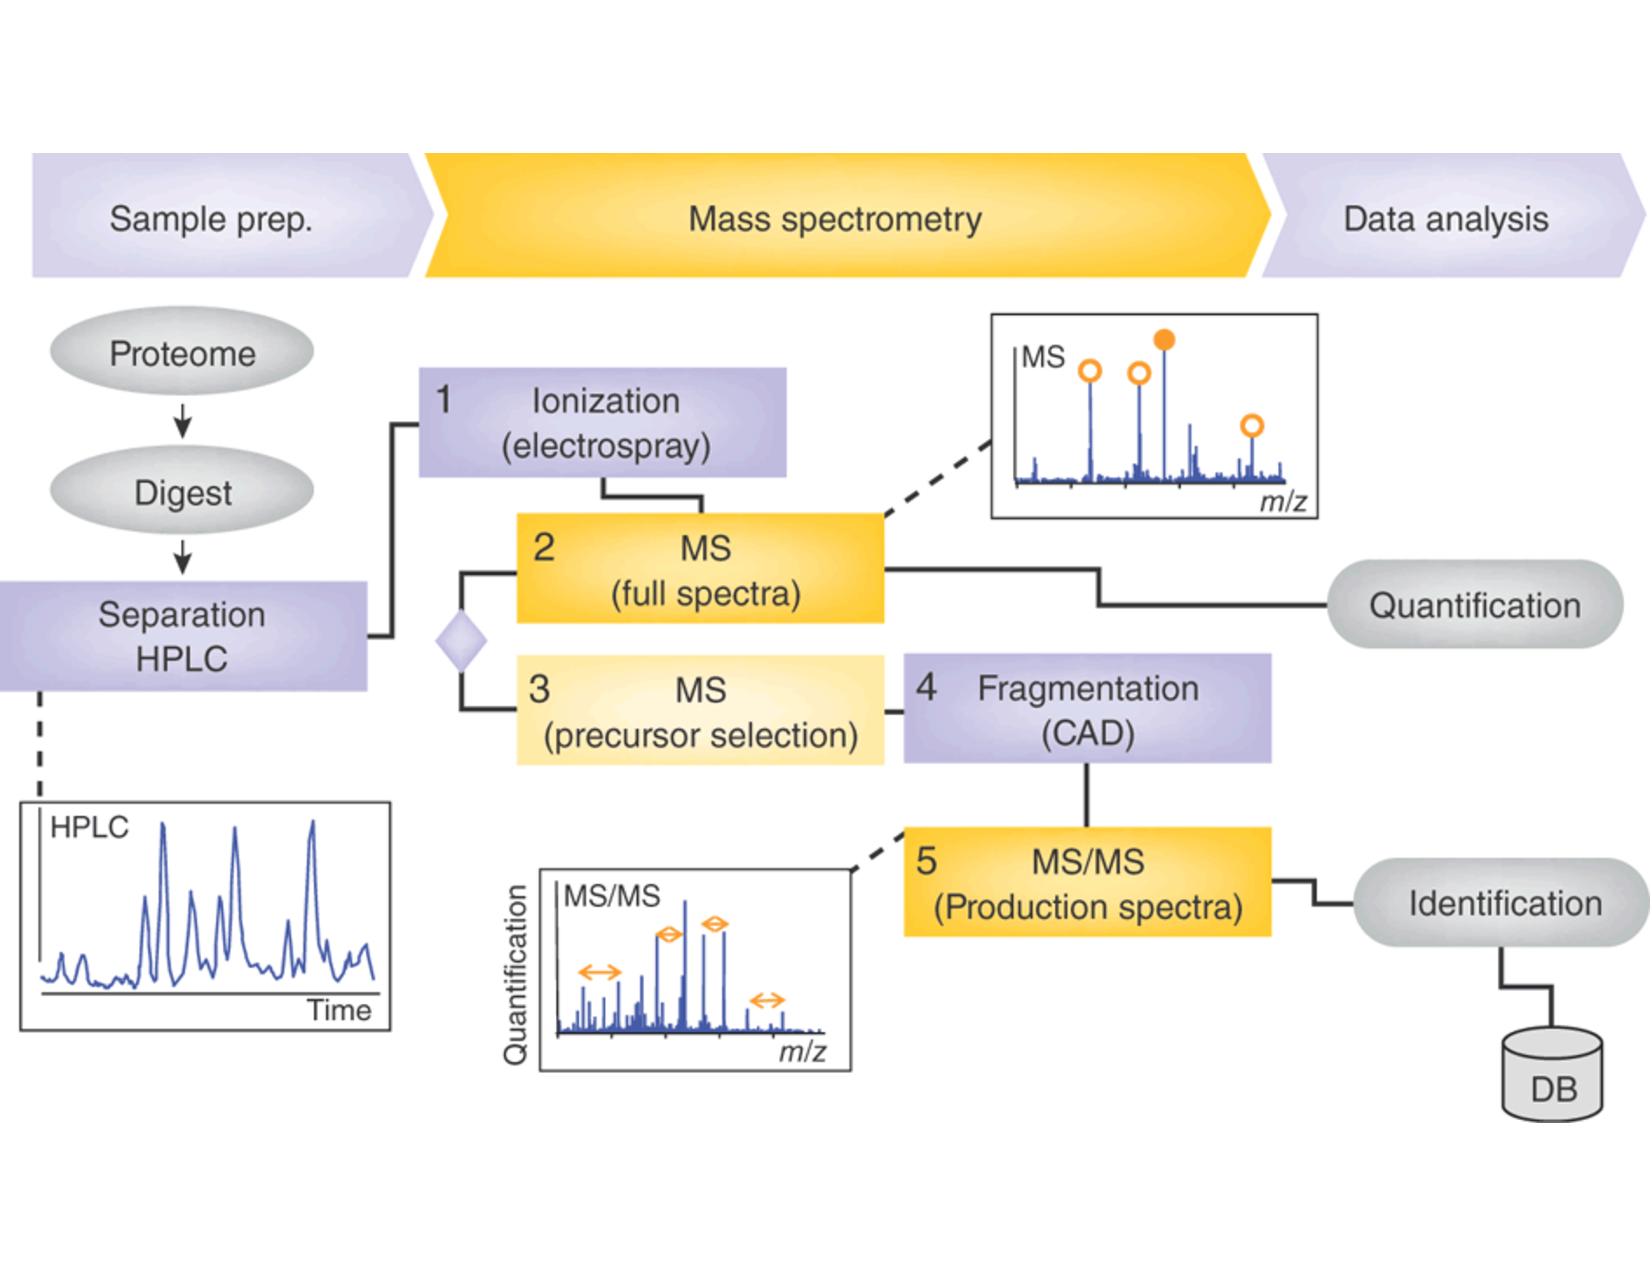
\includegraphics[width=10.5cm]{imagenes/WF}
\end{center}
\begin{center}
Secuenciación de alto rendimiento de proteomas
\end{center}
\end{frame}
\begin{frame}
\frametitle{Espectros de masas}
\begin{center}
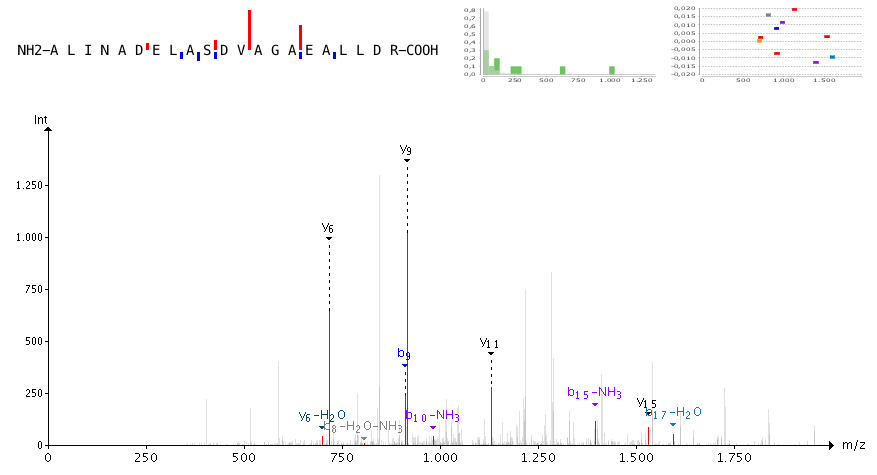
\includegraphics[width=11cm]{imagenes/Espectro}
\end{center}
\begin{center}
Representa la abundancia de los diferentes tipos de iones en función de la relación masa/carga de cada uno de ellos.
\end{center}
\end{frame}
\begin{frame}
\frametitle{Archivos *.MGF}
\texttt{
\\
TITLE=01-02.734.734.3 File:``01-02.RAW", NativeID:``controllerType=0 controllerNumber=1 scan=734"\\
BEGIN IONS\\
RTINSECONDS=810.6452\\
PEPMASS=423.252593994141 12337.3798828125\\
CHARGE=3+\\
129.1288300 52.872806549 \\
149.1461182 3.9003605843 \\
157.1478424 2.5976366997 \\
163.1104431 7.5093927383 \\
174.8226013 9.9194545746 \\
193.2301788 2.1630632877 \\
.\\
.\\
.\\
}
\end{frame}
\begin{frame}
\frametitle{Proteómica}
\begin{center}
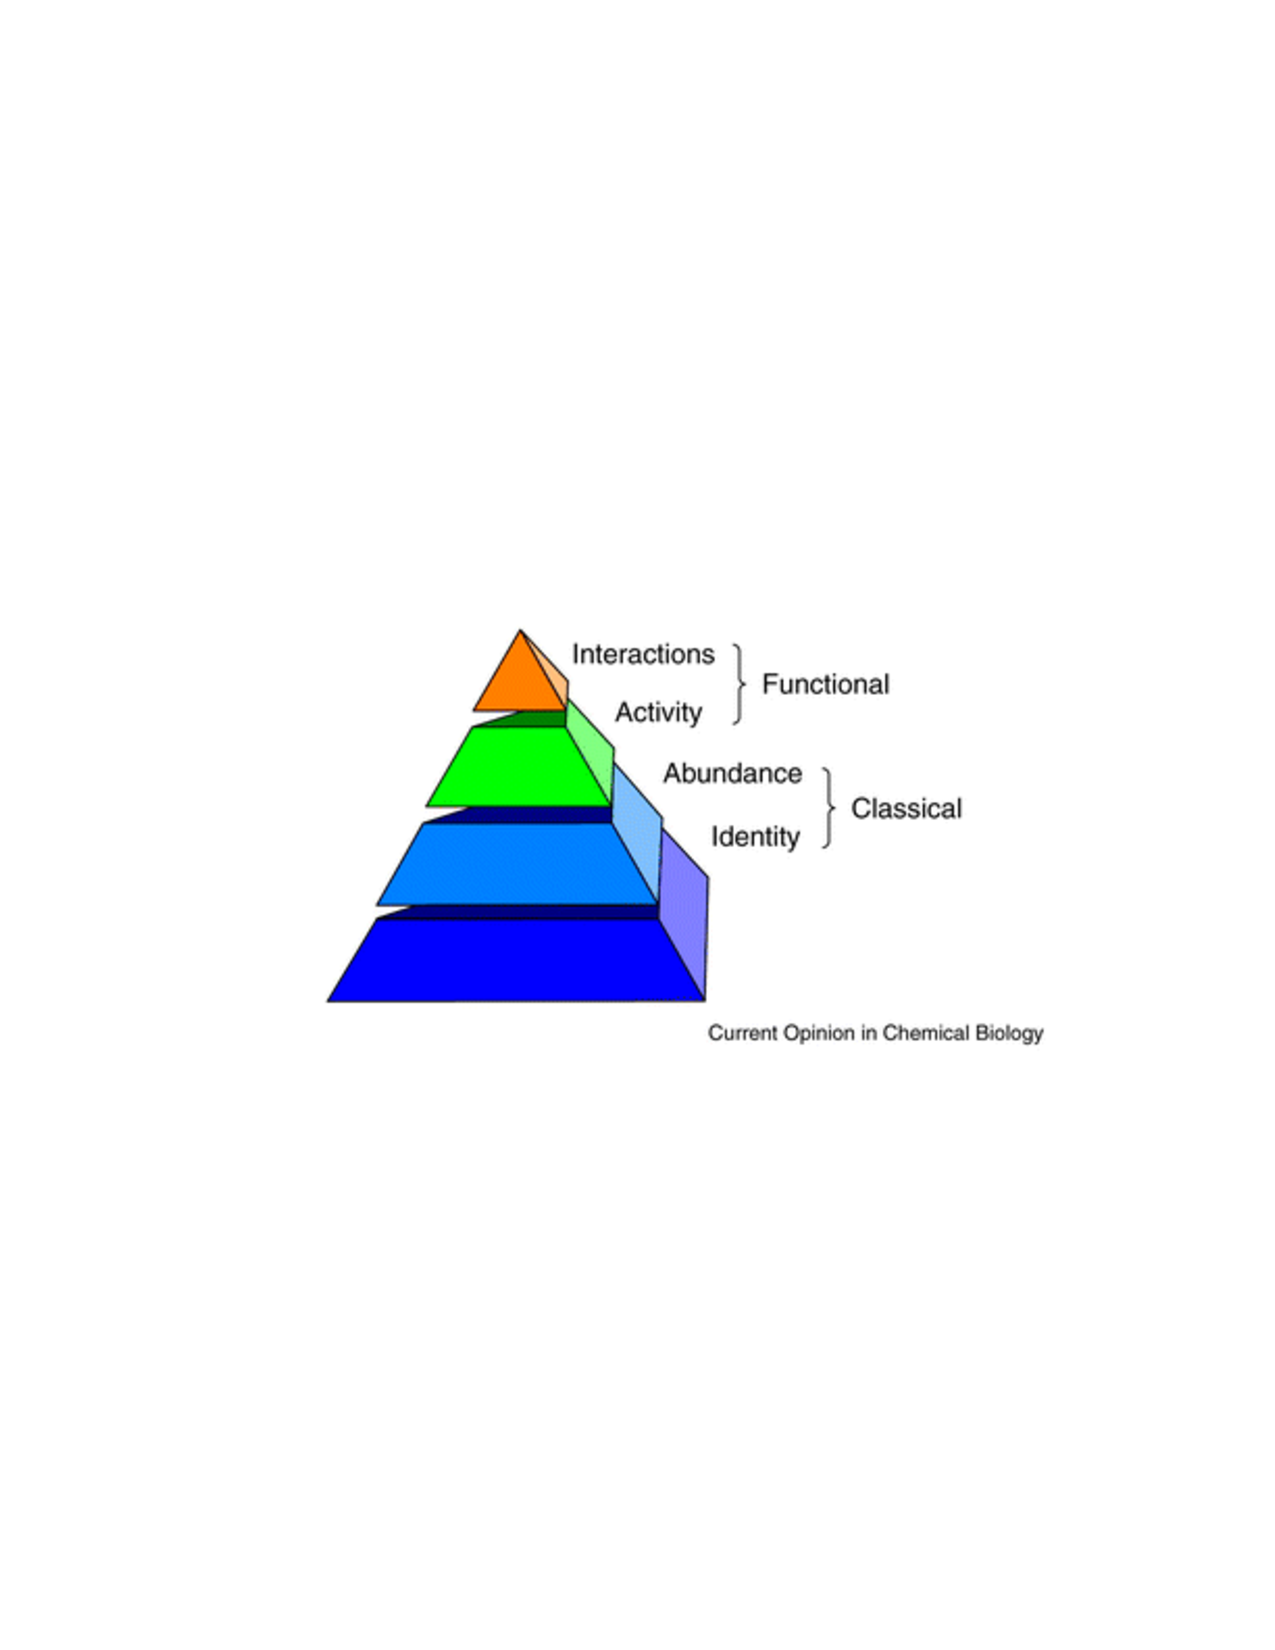
\includegraphics[width=8cm]{imagenes/Proteomics}
\end{center}
\begin{itemize}
\item La \emph{proteómica} es el estudio a gran escala de la identidad, abundancia, actividad e interacciones de las proteínas.
\pause
\item La comparación de proteomas en diferentes situaciones metabólicas permite identificar proteínas correlacionadas con determinados estadios fisiológicos.
\end{itemize}
\end{frame}
\begin{frame}
\frametitle{Objetivo:}
\begin{center}
\emph{Caracterizar computacionalmente el conjunto de proteínas expresadas diferencialmente} por el aumento en la concentración de ácidos grasos libres y la presencia del esteroide Tibolona en astrocitos humanos.
\end{center}
\end{frame}
\begin{frame}
\frametitle{Proteomics}
\begin{center}
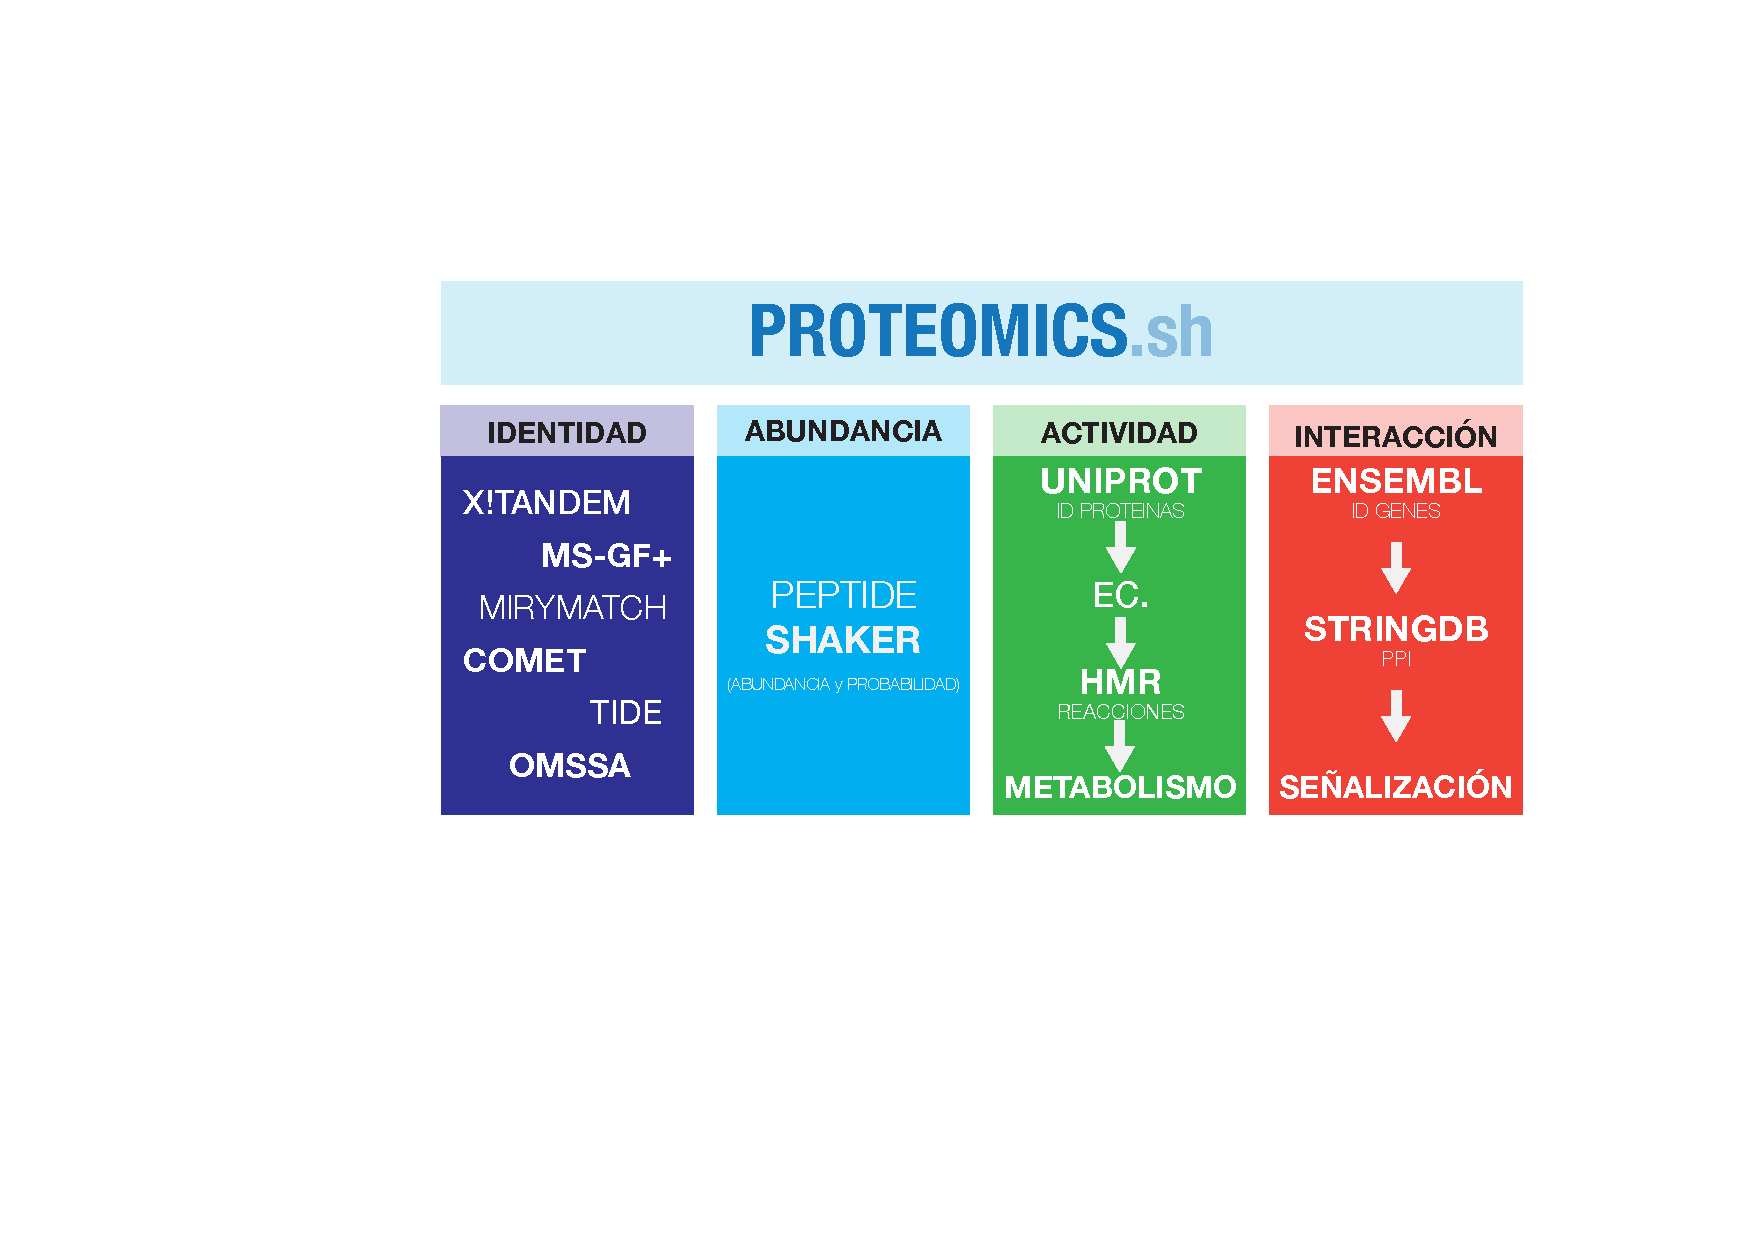
\includegraphics[width=11cm]{imagenes/PUJ-Proteomics}
\end{center}
\end{frame}
\begin{frame}
\frametitle{Prueba Piloto}
\begin{center}
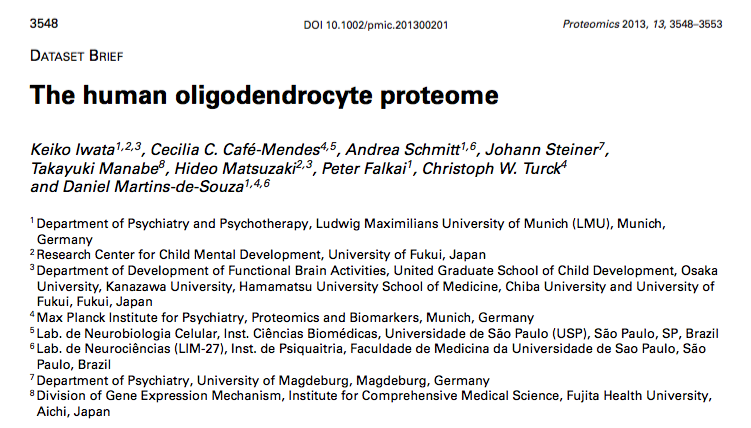
\includegraphics[width=11cm]{imagenes/OL}
\end{center}
\end{frame}
\begin{frame}
\frametitle{Motores de búsqueda}
\begin{center}

\includegraphics[height=0.8cm]{imagenes/logo_linux}\\
6 PARALELIZABLES, AUTOMATIZABLES Y DISEÑADOS PARA LINUX\\
\end{center}
\pause
\begin{center}
\begin{tabular}{ccc}
{\huge \textbf{MS-GF+}}&{\huge MYRIMATCH}&{\huge \textbf{OMSSA}}\\
{\huge X!TANDEM}&{\huge \textbf{COMET}}&{\huge TIDE}\\
\end{tabular}
\end{center}
\pause
\begin{center}
\begin{tabular}{|c|c|c|c|c|}
\hline
TIEMPO&PROTEINAS&PEPTIDES&P. CONFIABLES & P. DUDOSAS\\
\hline
\end{tabular}
\end{center}
\end{frame}
\begin{frame}
\frametitle{Selección de motores de búsqueda: PCA}
\begin{center}
\textbf{MODELO:} $CONFPROT + CONFIDENT + INVTIME$
\end{center}
\begin{center}
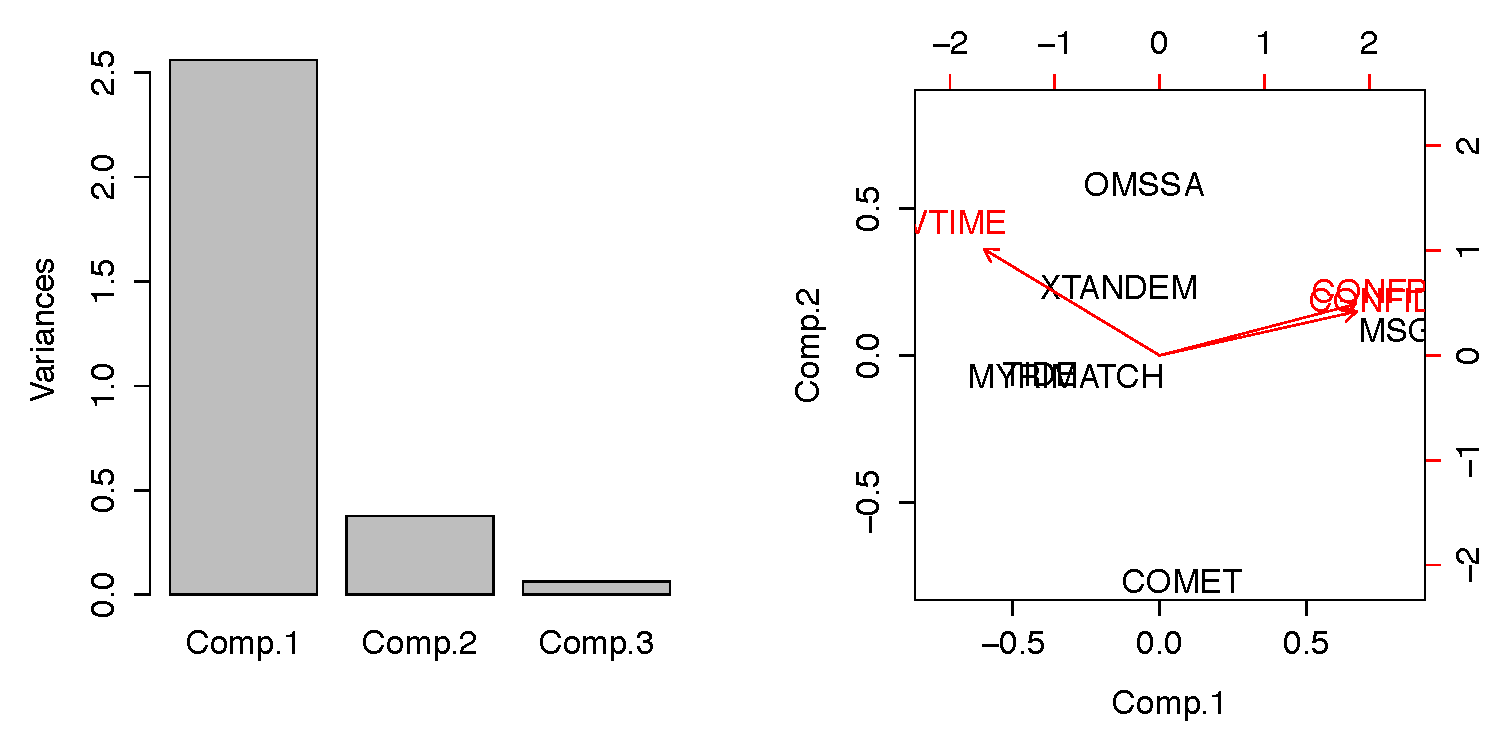
\includegraphics[width=10cm]{imagenes/PCA}
\end{center}
\end{frame}
\begin{frame}
\frametitle{Selección de motores de búsqueda}
\begin{center}
\textbf{SELECCIONADOS:} MSGF + COMET + OMSSA 
\end{center}
\begin{center}
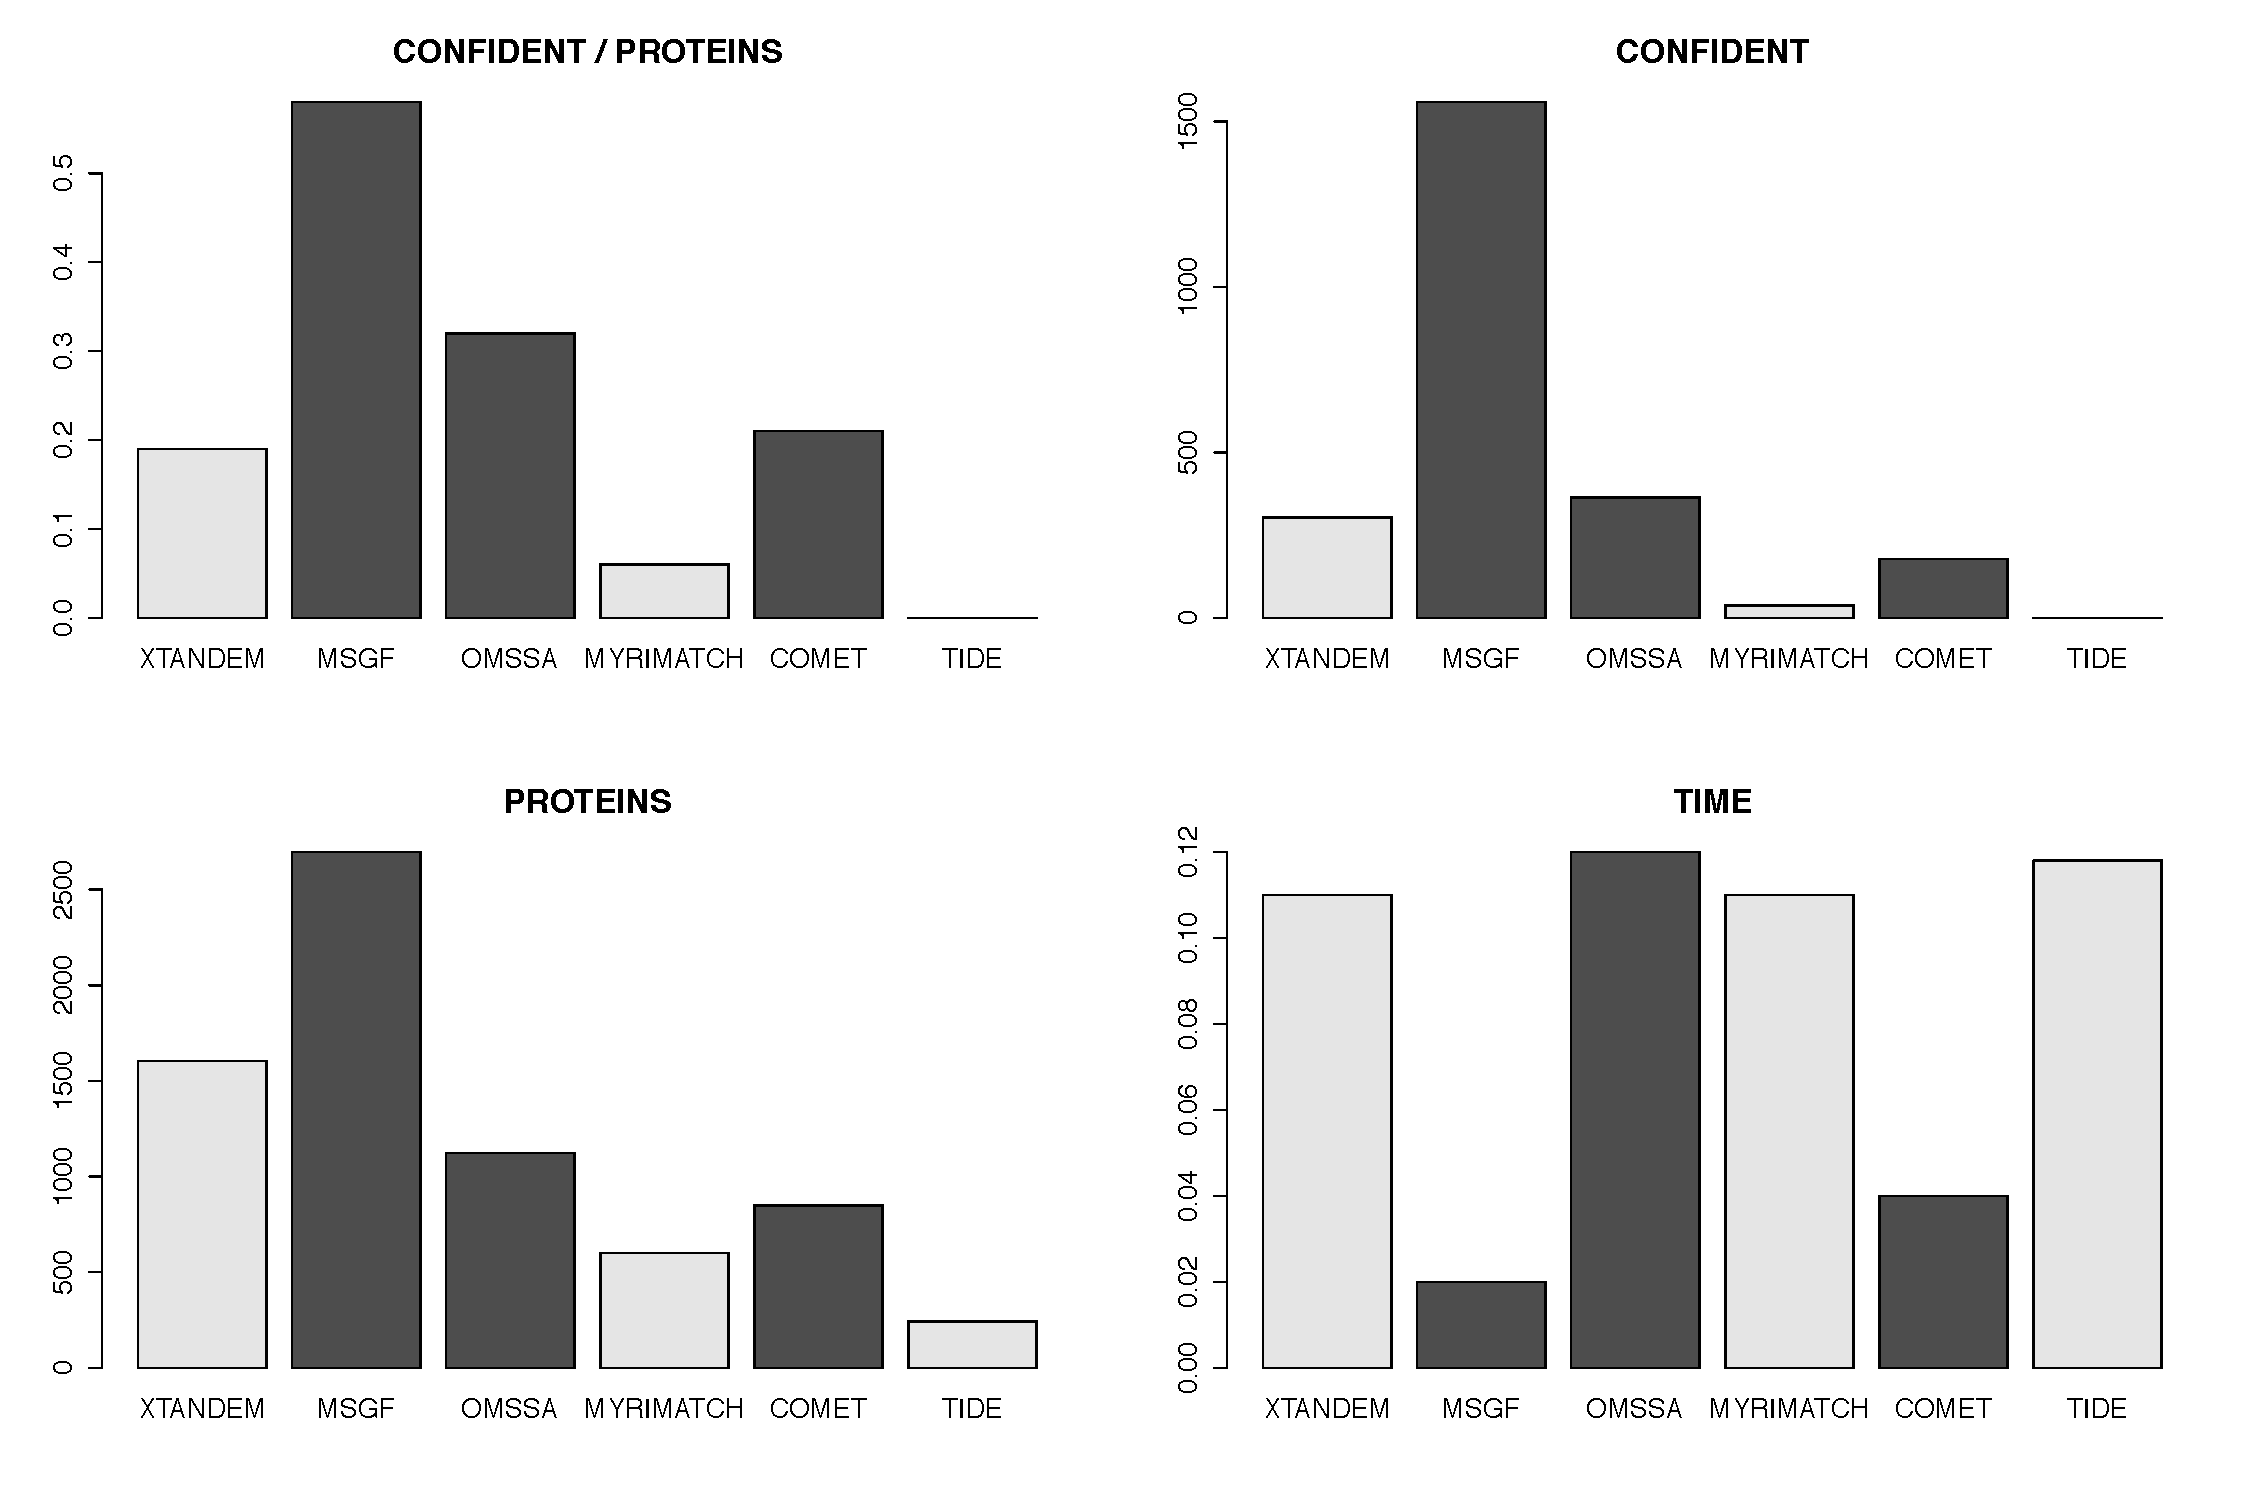
\includegraphics[width=10cm]{imagenes/ENGINES}\\
\textbf{TOTAL PROTEÍNAS IDENTIFICADAS}: 2696
\end{center}
\end{frame}
\begin{frame}
\frametitle{Proteínas identificadas}
\begin{center}
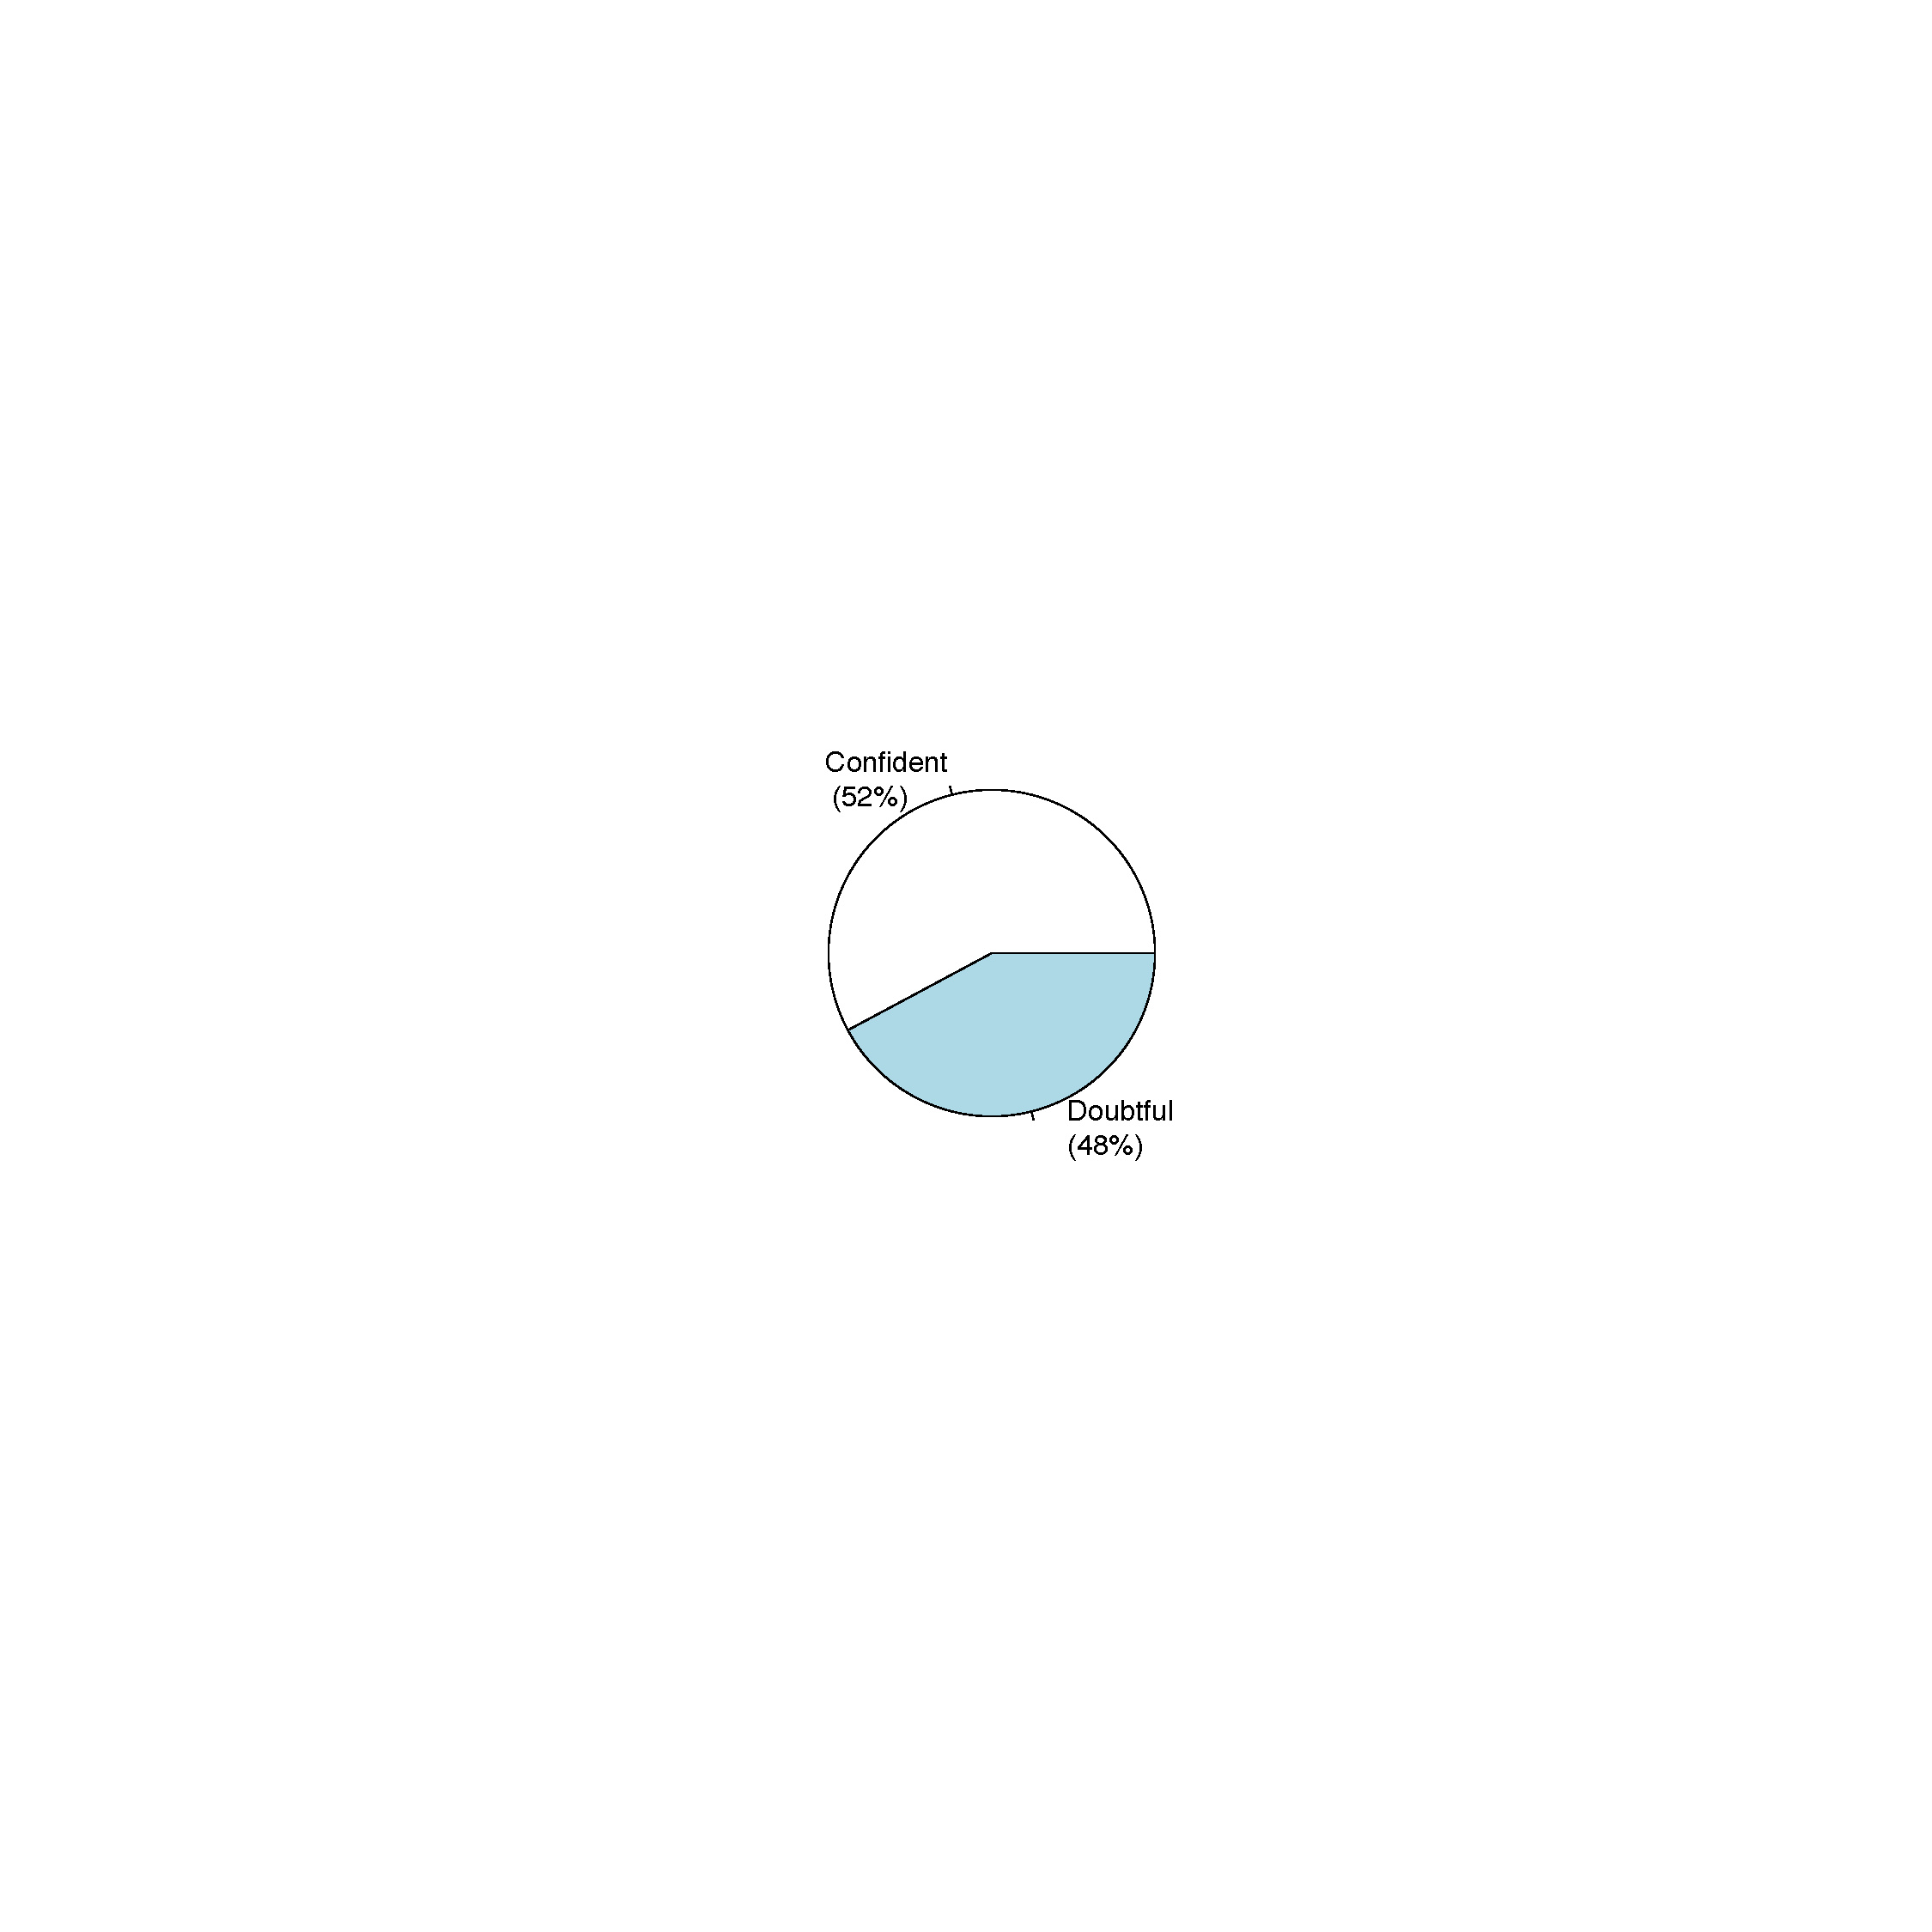
\includegraphics[width=6cm]{imagenes/Proteins}
\end{center}
\begin{center}
\textbf{CONFIABLE:} PSM/Proteína, Base de datos objetivo, FDR < 1\%.
\end{center}
\end{frame}
\begin{frame}
\frametitle{Proteínas identificadas}
\begin{center}
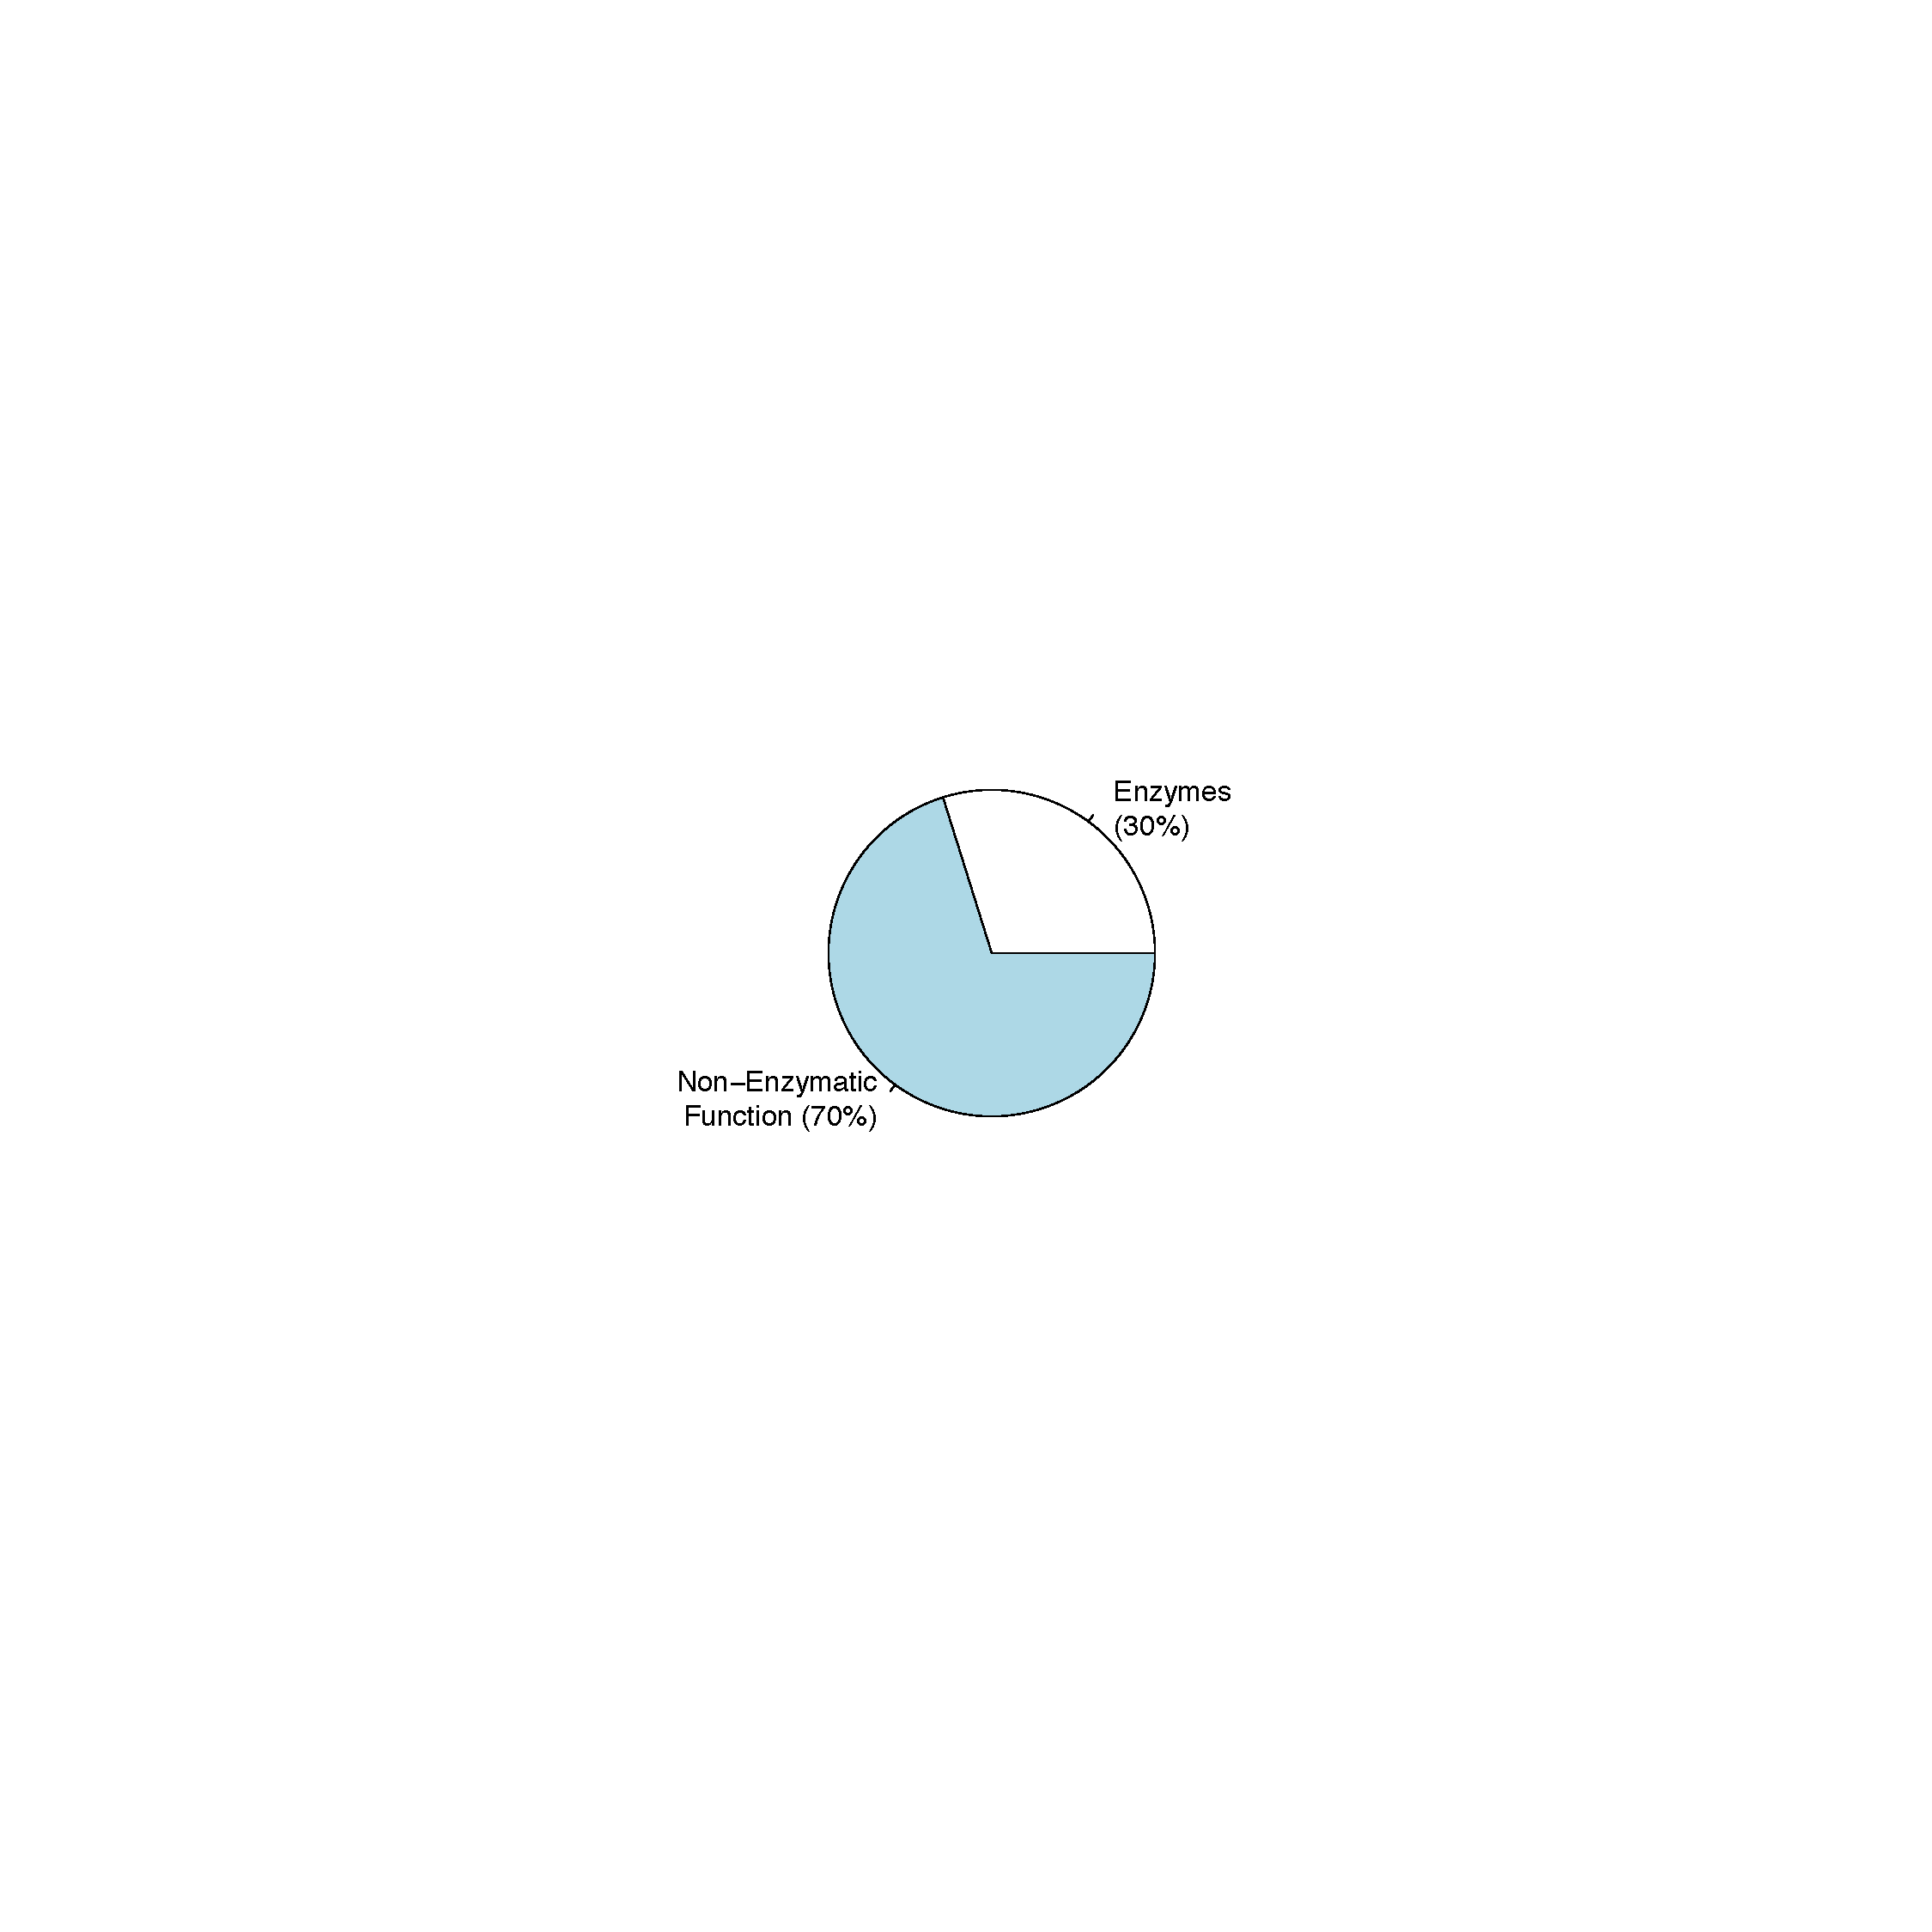
\includegraphics[width=10cm]{imagenes/ECProt}
\end{center}
\begin{center}
\textbf{ENZIMA:} Número EC. asociado al ID de la Proteína en UNIPROT
\end{center}
\end{frame}
\begin{frame}
\frametitle{Proteínas identificadas}
\begin{center}
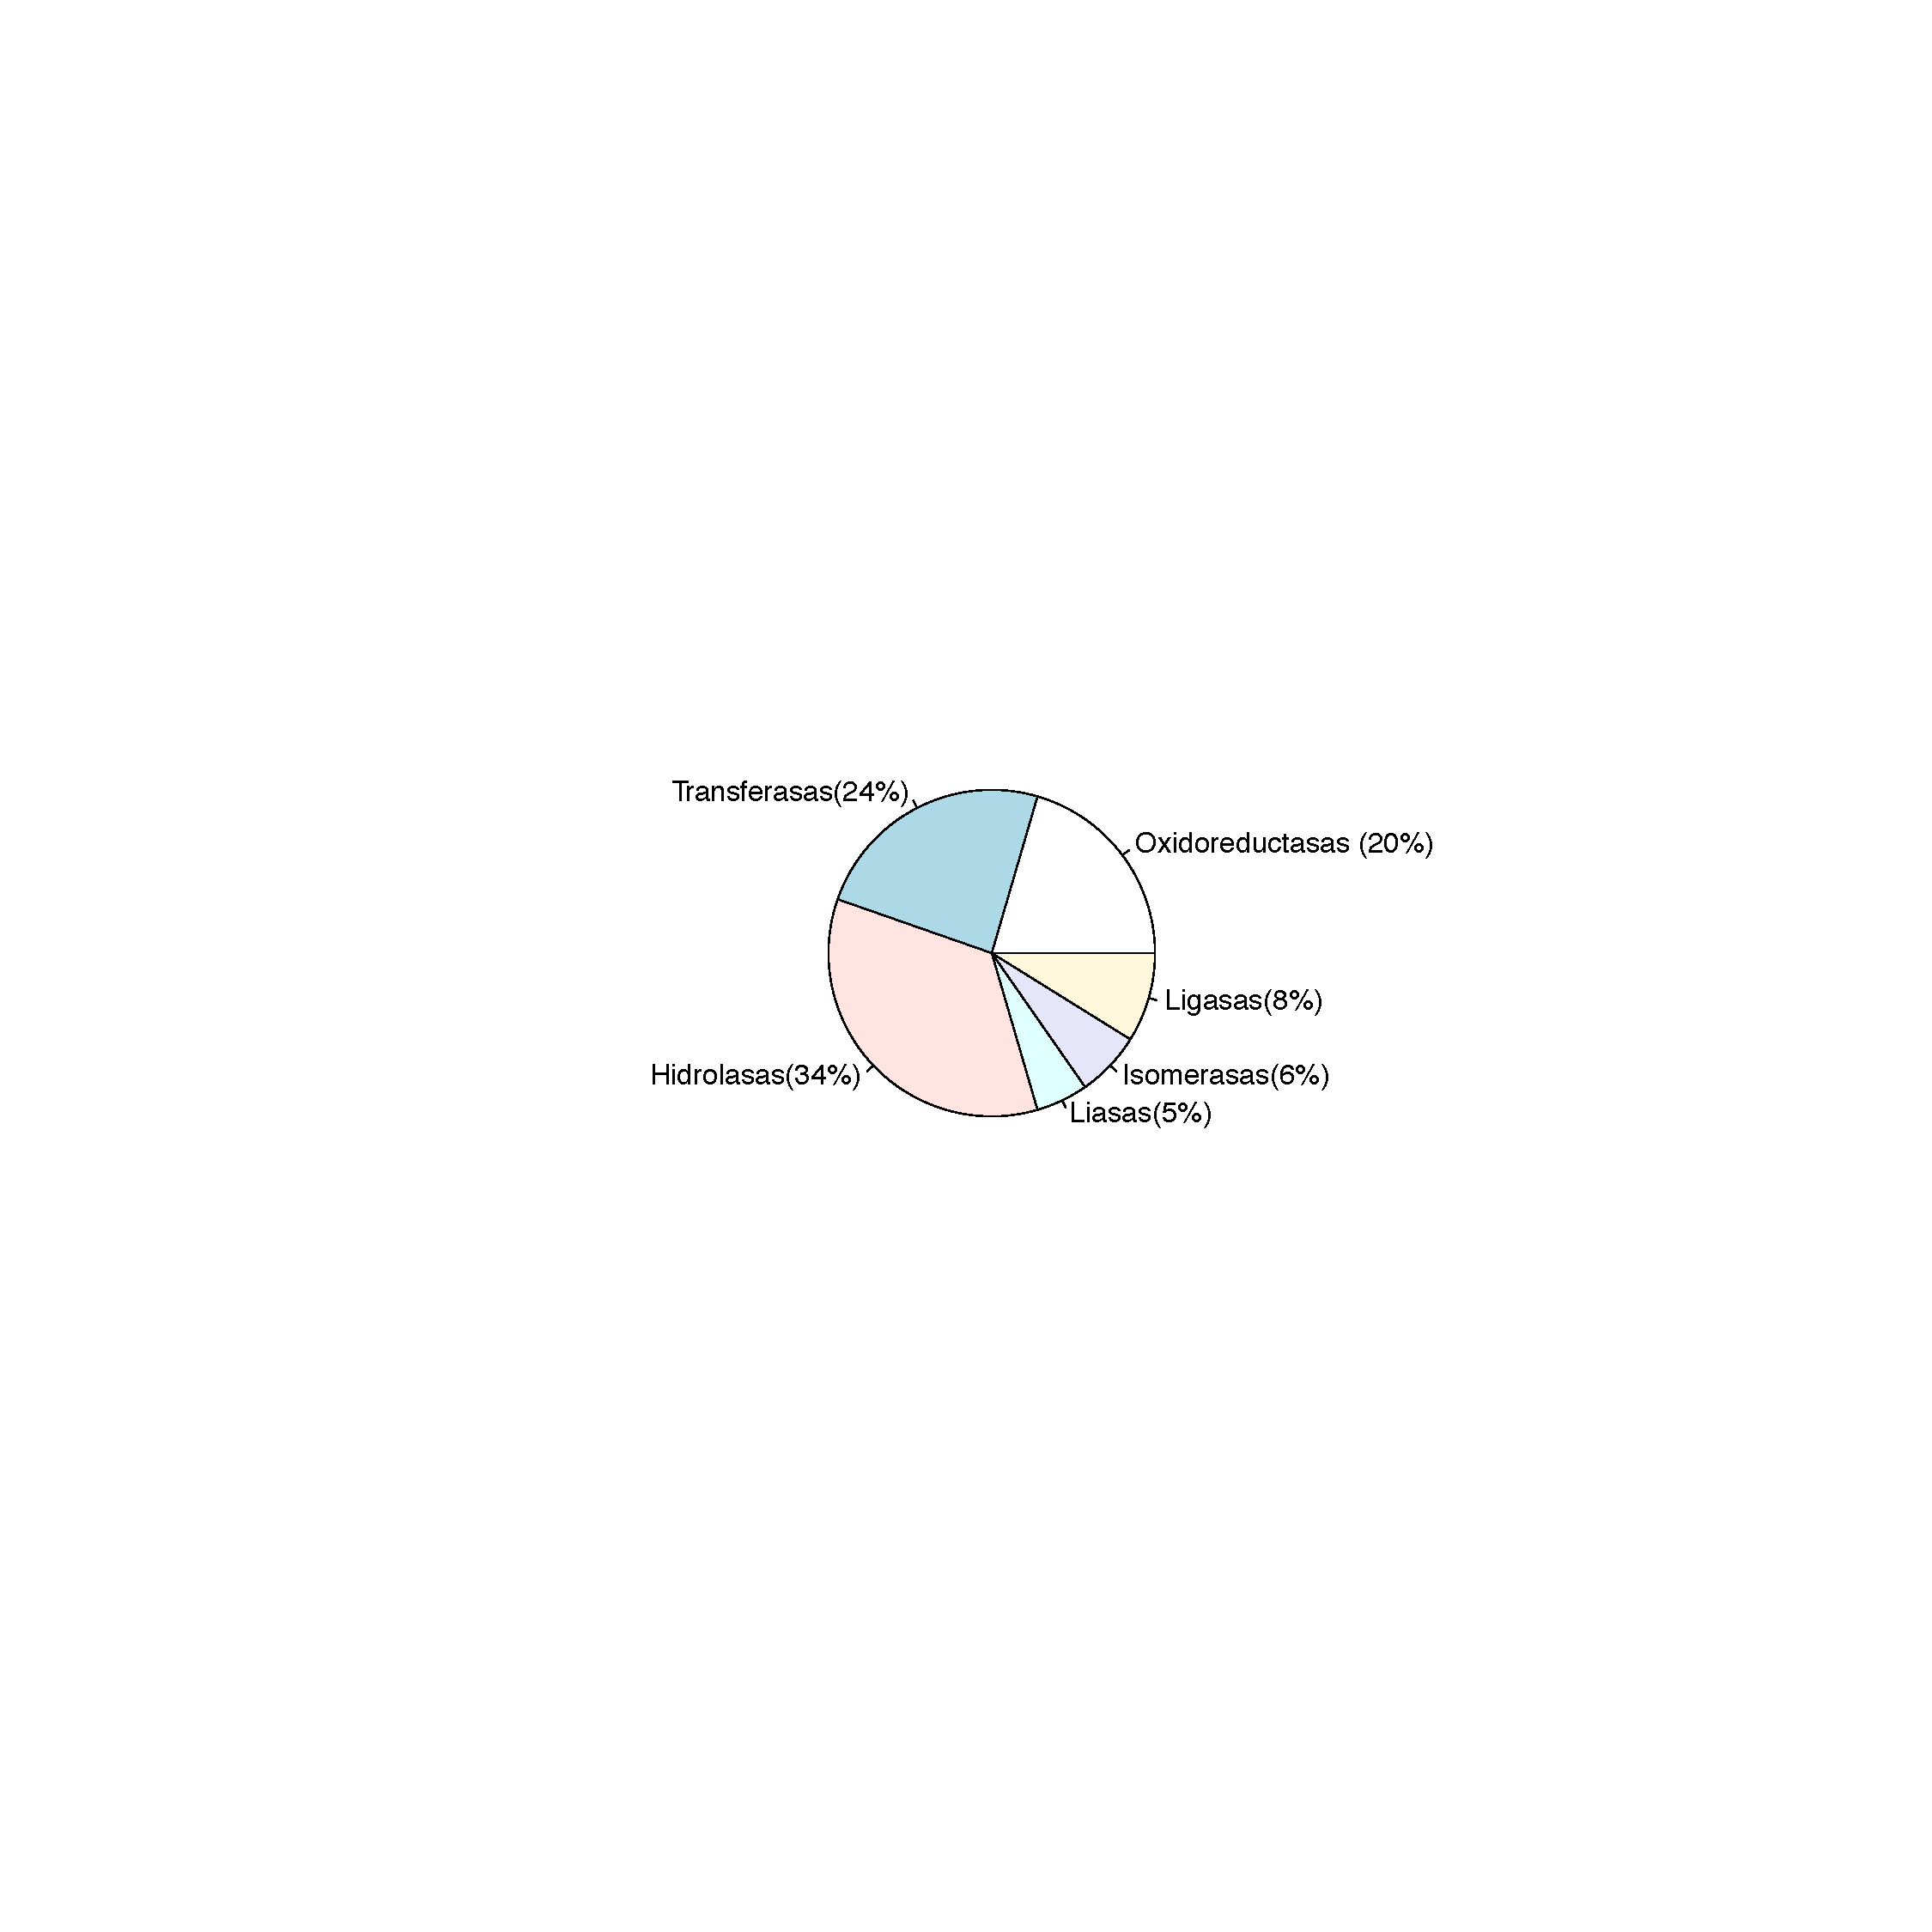
\includegraphics[width=10cm]{imagenes/ECN}
\end{center}
\begin{center}
Funciones Enzimáticas
\end{center}
\end{frame}
\begin{frame}
\frametitle{Reconstrucciones metabólicas}
\begin{center}
\begin{tabular}{|c|c|c|}
\hline
\multicolumn{3}{|c|}{\textbf{REDES}}\\
\hline
\hline
REGULACIÓN&SEÑALIZACIÓN&METABOLISMO\\
\hline
\textbf{PROT-DNA}&\textbf{PROT-PROT}& \textbf{ENZIMAS} \\
\hline
\end{tabular}
\end{center}
\end{frame}
\begin{frame}
\frametitle{Redes Metabólicas}
\begin{center}
\includegraphics[width=10.5cm]{imagenes/Met}
\end{center}
\begin{center}
465\textbf{:ENZIMAS} 541\textbf{:FUNCIONES ENZIMÁTICAS} 4190\textbf{:REACCIONES} 109\textbf{:RUTAS}
\end{center}
\end{frame}
\plain{¿preguntas?}
\end{document}
